\documentclass[twoside]{book}

% Packages required by doxygen
\usepackage{fixltx2e}
\usepackage{calc}
\usepackage{doxygen}
\usepackage[export]{adjustbox} % also loads graphicx
\usepackage{graphicx}
\usepackage[utf8]{inputenc}
\usepackage{makeidx}
\usepackage{multicol}
\usepackage{multirow}
\PassOptionsToPackage{warn}{textcomp}
\usepackage{textcomp}
\usepackage[nointegrals]{wasysym}
\usepackage[table]{xcolor}

% Font selection
\usepackage[T1]{fontenc}
\usepackage[scaled=.90]{helvet}
\usepackage{courier}
\usepackage{amssymb}
\usepackage{sectsty}
\renewcommand{\familydefault}{\sfdefault}
\allsectionsfont{%
  \fontseries{bc}\selectfont%
  \color{darkgray}%
}
\renewcommand{\DoxyLabelFont}{%
  \fontseries{bc}\selectfont%
  \color{darkgray}%
}
\newcommand{\+}{\discretionary{\mbox{\scriptsize$\hookleftarrow$}}{}{}}

% Page & text layout
\usepackage{geometry}
\geometry{%
  a4paper,%
  top=2.5cm,%
  bottom=2.5cm,%
  left=2.5cm,%
  right=2.5cm%
}
\tolerance=750
\hfuzz=15pt
\hbadness=750
\setlength{\emergencystretch}{15pt}
\setlength{\parindent}{0cm}
\setlength{\parskip}{3ex plus 2ex minus 2ex}
\makeatletter
\renewcommand{\paragraph}{%
  \@startsection{paragraph}{4}{0ex}{-1.0ex}{1.0ex}{%
    \normalfont\normalsize\bfseries\SS@parafont%
  }%
}
\renewcommand{\subparagraph}{%
  \@startsection{subparagraph}{5}{0ex}{-1.0ex}{1.0ex}{%
    \normalfont\normalsize\bfseries\SS@subparafont%
  }%
}
\makeatother

% Headers & footers
\usepackage{fancyhdr}
\pagestyle{fancyplain}
\fancyhead[LE]{\fancyplain{}{\bfseries\thepage}}
\fancyhead[CE]{\fancyplain{}{}}
\fancyhead[RE]{\fancyplain{}{\bfseries\leftmark}}
\fancyhead[LO]{\fancyplain{}{\bfseries\rightmark}}
\fancyhead[CO]{\fancyplain{}{}}
\fancyhead[RO]{\fancyplain{}{\bfseries\thepage}}
\fancyfoot[LE]{\fancyplain{}{}}
\fancyfoot[CE]{\fancyplain{}{}}
\fancyfoot[RE]{\fancyplain{}{\bfseries\scriptsize Generated by Doxygen }}
\fancyfoot[LO]{\fancyplain{}{\bfseries\scriptsize Generated by Doxygen }}
\fancyfoot[CO]{\fancyplain{}{}}
\fancyfoot[RO]{\fancyplain{}{}}
\renewcommand{\footrulewidth}{0.4pt}
\renewcommand{\chaptermark}[1]{%
  \markboth{#1}{}%
}
\renewcommand{\sectionmark}[1]{%
  \markright{\thesection\ #1}%
}

% Indices & bibliography
\usepackage{natbib}
\usepackage[titles]{tocloft}
\setcounter{tocdepth}{3}
\setcounter{secnumdepth}{5}
\makeindex

% Hyperlinks (required, but should be loaded last)
\usepackage{ifpdf}
\ifpdf
  \usepackage[pdftex,pagebackref=true]{hyperref}
\else
  \usepackage[ps2pdf,pagebackref=true]{hyperref}
\fi
\hypersetup{%
  colorlinks=true,%
  linkcolor=blue,%
  citecolor=blue,%
  unicode%
}

% Custom commands
\newcommand{\clearemptydoublepage}{%
  \newpage{\pagestyle{empty}\cleardoublepage}%
}

\usepackage{caption}
\captionsetup{labelsep=space,justification=centering,font={bf},singlelinecheck=off,skip=4pt,position=top}

%===== C O N T E N T S =====

\begin{document}

% Titlepage & ToC
\hypersetup{pageanchor=false,
             bookmarksnumbered=true,
             pdfencoding=unicode
            }
\pagenumbering{alph}
\begin{titlepage}
\vspace*{7cm}
\begin{center}%
{\Large R\+C\+Plane \\[1ex]\large 0.\+1 }\\
\vspace*{1cm}
{\large Generated by Doxygen 1.8.13}\\
\end{center}
\end{titlepage}
\clearemptydoublepage
\pagenumbering{roman}
\tableofcontents
\clearemptydoublepage
\pagenumbering{arabic}
\hypersetup{pageanchor=true}

%--- Begin generated contents ---
\chapter{Class Index}
\section{Class List}
Here are the classes, structs, unions and interfaces with brief descriptions\+:\begin{DoxyCompactList}
\item\contentsline{section}{\hyperlink{class_battery}{Battery} }{\pageref{class_battery}}{}
\item\contentsline{section}{\hyperlink{classbattery}{battery} \\*Represents the Lipo battery pack and implements methods to get its charge level }{\pageref{classbattery}}{}
\item\contentsline{section}{\hyperlink{class_button}{Button} \\*\hyperlink{class_button}{Button} class is responsible for reading a pushbutton state with debounce feature }{\pageref{class_button}}{}
\item\contentsline{section}{\hyperlink{class_buzzer}{Buzzer} \\*\hyperlink{class_buzzer}{Buzzer} class is responsible for sound outputs }{\pageref{class_buzzer}}{}
\item\contentsline{section}{\hyperlink{class_control}{Control} \\*\hyperlink{class_control}{Control} class is responsible for translating \hyperlink{class_joystick}{Joystick}, encoder and button inputs into power, pitch, yaw and roll values }{\pageref{class_control}}{}
\item\contentsline{section}{\hyperlink{class_encoder}{Encoder} \\*\hyperlink{class_encoder}{Encoder} class is responsible for reading rotary encoder input }{\pageref{class_encoder}}{}
\item\contentsline{section}{\hyperlink{class_joystick}{Joystick} }{\pageref{class_joystick}}{}
\item\contentsline{section}{\hyperlink{class_l_c_d_screen}{L\+C\+D\+Screen} \\*\hyperlink{class_l_c_d_screen}{L\+C\+D\+Screen} class is responsible for displaying informations on an S\+S\+D1306 I2C screen }{\pageref{class_l_c_d_screen}}{}
\item\contentsline{section}{\hyperlink{class_led}{Led} }{\pageref{class_led}}{}
\item\contentsline{section}{\hyperlink{class_plane_battery_bisplay}{Plane\+Battery\+Bisplay} \\*Responsible for displaying battery informations }{\pageref{class_plane_battery_bisplay}}{}
\item\contentsline{section}{\hyperlink{struct_pto_t_data_frame}{Pto\+T\+Data\+Frame} \\*Struct composed with all data contained in a frame sent from the Plane to the Transmitter }{\pageref{struct_pto_t_data_frame}}{}
\item\contentsline{section}{\hyperlink{class_radio}{Radio} \\*\hyperlink{class_radio}{Radio} class responsible for communicating with the \hyperlink{class_radio}{Radio} Transmitter on the ground }{\pageref{class_radio}}{}
\item\contentsline{section}{\hyperlink{class_remote_battery}{Remote\+Battery} }{\pageref{class_remote_battery}}{}
\item\contentsline{section}{\hyperlink{class_r_g_b_led}{R\+G\+B\+Led} \\*\hyperlink{class_r_g_b_led}{R\+G\+B\+Led} class is responsible for displaying colors on an R\+GB \hyperlink{class_led}{Led} }{\pageref{class_r_g_b_led}}{}
\item\contentsline{section}{\hyperlink{class_settings}{Settings} \\*\hyperlink{class_settings}{Settings} class is responsible for }{\pageref{class_settings}}{}
\item\contentsline{section}{\hyperlink{class_sevseg_screen}{Sevseg\+Screen} \\*\hyperlink{class_sevseg_screen}{Sevseg\+Screen} class is responsible for displaying content on a 7-\/segment display }{\pageref{class_sevseg_screen}}{}
\item\contentsline{section}{\hyperlink{class_switch}{Switch} }{\pageref{class_switch}}{}
\item\contentsline{section}{\hyperlink{struct_tto_p_data_frame}{Tto\+P\+Data\+Frame} \\*Struct composed with all data contained in a frame sent from the Transmitter to the Plane }{\pageref{struct_tto_p_data_frame}}{}
\end{DoxyCompactList}

\chapter{File Index}
\section{File List}
Here is a list of all documented files with brief descriptions\+:\begin{DoxyCompactList}
\item\contentsline{section}{src/main/\hyperlink{battery_8cpp}{battery.\+cpp} \\*Definition of battery class }{\pageref{battery_8cpp}}{}
\item\contentsline{section}{src/main/\hyperlink{battery_8h}{battery.\+h} \\*Declaration of battery class }{\pageref{battery_8h}}{}
\item\contentsline{section}{src/main/\hyperlink{button_8cpp}{button.\+cpp} \\*Definition of \hyperlink{class_button}{Button} class }{\pageref{button_8cpp}}{}
\item\contentsline{section}{src/main/\hyperlink{button_8h}{button.\+h} \\*Declaration of \hyperlink{class_button}{Button} class }{\pageref{button_8h}}{}
\item\contentsline{section}{src/main/\hyperlink{buzzer_8cpp}{buzzer.\+cpp} \\*Definition of buzzer class }{\pageref{buzzer_8cpp}}{}
\item\contentsline{section}{src/main/\hyperlink{buzzer_8h}{buzzer.\+h} \\*Declaration of \hyperlink{class_buzzer}{Buzzer} class }{\pageref{buzzer_8h}}{}
\item\contentsline{section}{src/main/\hyperlink{control_8cpp}{control.\+cpp} \\*Definition of control class }{\pageref{control_8cpp}}{}
\item\contentsline{section}{src/main/\hyperlink{control_8h}{control.\+h} \\*Declaration of control class }{\pageref{control_8h}}{}
\item\contentsline{section}{src/main/\hyperlink{encoder_8cpp}{encoder.\+cpp} \\*Definition of \hyperlink{class_encoder}{Encoder} class }{\pageref{encoder_8cpp}}{}
\item\contentsline{section}{src/main/\hyperlink{encoder_8h}{encoder.\+h} \\*Declaration of \hyperlink{class_encoder}{Encoder} class }{\pageref{encoder_8h}}{}
\item\contentsline{section}{src/main/\hyperlink{frame_8h}{frame.\+h} \\*Declaration of frame types and incoming\+Frame class }{\pageref{frame_8h}}{}
\item\contentsline{section}{src/main/{\bfseries header.\+h} }{\pageref{header_8h}}{}
\item\contentsline{section}{src/main/\hyperlink{joystick_8cpp}{joystick.\+cpp} \\*Definition of \hyperlink{class_joystick}{Joystick} class }{\pageref{joystick_8cpp}}{}
\item\contentsline{section}{src/main/\hyperlink{joystick_8h}{joystick.\+h} \\*Declaration of \hyperlink{class_joystick}{Joystick} class }{\pageref{joystick_8h}}{}
\item\contentsline{section}{src/main/\hyperlink{lcd__bitmaps_8h}{lcd\+\_\+bitmaps.\+h} \\*Contain arrays describing btmaps do display on main L\+CD }{\pageref{lcd__bitmaps_8h}}{}
\item\contentsline{section}{src/main/\hyperlink{lcdscreen_8cpp}{lcdscreen.\+cpp} \\*Definition of \hyperlink{class_l_c_d_screen}{L\+C\+D\+Screen} class }{\pageref{lcdscreen_8cpp}}{}
\item\contentsline{section}{src/main/\hyperlink{lcdscreen_8h}{lcdscreen.\+h} \\*Declaration of \hyperlink{class_l_c_d_screen}{L\+C\+D\+Screen} class }{\pageref{lcdscreen_8h}}{}
\item\contentsline{section}{src/main/\hyperlink{led_8cpp}{led.\+cpp} \\*Definition of \hyperlink{class_led}{Led} class }{\pageref{led_8cpp}}{}
\item\contentsline{section}{src/main/\hyperlink{led_8h}{led.\+h} \\*Declaration of \hyperlink{class_led}{Led} class }{\pageref{led_8h}}{}
\item\contentsline{section}{src/main/\hyperlink{math_functions_8h}{math\+Functions.\+h} \\*Declaration of a set of mathematical functions }{\pageref{math_functions_8h}}{}
\item\contentsline{section}{src/main/{\bfseries plane\+\_\+battery\+\_\+display.\+h} }{\pageref{plane__battery__display_8h}}{}
\item\contentsline{section}{src/main/\hyperlink{radio_8cpp}{radio.\+cpp} \\*Definition of radio class }{\pageref{radio_8cpp}}{}
\item\contentsline{section}{src/main/\hyperlink{radio_8h}{radio.\+h} \\*Declaration of radio class }{\pageref{radio_8h}}{}
\item\contentsline{section}{src/main/{\bfseries remote\+\_\+battery.\+h} }{\pageref{remote__battery_8h}}{}
\item\contentsline{section}{src/main/\hyperlink{rgbled_8cpp}{rgbled.\+cpp} \\*Definition of \hyperlink{class_r_g_b_led}{R\+G\+B\+Led} class }{\pageref{rgbled_8cpp}}{}
\item\contentsline{section}{src/main/\hyperlink{rgbled_8h}{rgbled.\+h} \\*Declaration of \hyperlink{class_r_g_b_led}{R\+G\+B\+Led} class }{\pageref{rgbled_8h}}{}
\item\contentsline{section}{src/main/\hyperlink{settings_8cpp}{settings.\+cpp} \\*Definition of settings class }{\pageref{settings_8cpp}}{}
\item\contentsline{section}{src/main/\hyperlink{settings_8h}{settings.\+h} \\*Default settings and declaration of settings class }{\pageref{settings_8h}}{}
\item\contentsline{section}{src/main/\hyperlink{sevsegscreen_8cpp}{sevsegscreen.\+cpp} \\*Definition of \hyperlink{class_sevseg_screen}{Sevseg\+Screen} class }{\pageref{sevsegscreen_8cpp}}{}
\item\contentsline{section}{src/main/\hyperlink{sevsegscreen_8h}{sevsegscreen.\+h} \\*Declaration of \hyperlink{class_sevseg_screen}{Sevseg\+Screen} class }{\pageref{sevsegscreen_8h}}{}
\item\contentsline{section}{src/main/\hyperlink{switch_8h}{switch.\+h} \\*Declaration of switch class }{\pageref{switch_8h}}{}
\end{DoxyCompactList}

\chapter{Class Documentation}
\hypertarget{class_aileron}{}\section{Aileron Class Reference}
\label{class_aileron}\index{Aileron@{Aileron}}


Representation of the ailerons.  




{\ttfamily \#include $<$aileron.\+h$>$}

\subsection*{Public Member Functions}
\begin{DoxyCompactItemize}
\item 
void \hyperlink{class_aileron_ad28b0e5e53705b1f43a3fa73c0765a96}{init} (int pin\+\_\+p, int min\+\_\+p, int max\+\_\+p)
\begin{DoxyCompactList}\small\item\em Initialize the servomotor associated with the aileron. \end{DoxyCompactList}\item 
\mbox{\Hypertarget{class_aileron_a5d5579971f2679d708d01657d63da414}\label{class_aileron_a5d5579971f2679d708d01657d63da414}} 
void \hyperlink{class_aileron_a5d5579971f2679d708d01657d63da414}{reverse} ()
\begin{DoxyCompactList}\small\item\em reverses the current sense of rotation of the servomotor \end{DoxyCompactList}\item 
void \hyperlink{class_aileron_af05ea195df6881618c7835153537cba1}{move\+To} (uint8\+\_\+t position\+\_\+p)
\begin{DoxyCompactList}\small\item\em moves aileron with a given angle \end{DoxyCompactList}\item 
void \hyperlink{class_aileron_a02d1842c6782dbb43fd70d1e3669c960}{move\+Speed} (uint8\+\_\+t position\+\_\+p, uint8\+\_\+t speed\+\_\+p=100, int start\+\_\+p=-\/1)
\begin{DoxyCompactList}\small\item\em moves aileron at specified speed \end{DoxyCompactList}\item 
\mbox{\Hypertarget{class_aileron_abeee29a990a1a9b3d8bc884991b7221f}\label{class_aileron_abeee29a990a1a9b3d8bc884991b7221f}} 
void \hyperlink{class_aileron_abeee29a990a1a9b3d8bc884991b7221f}{move\+Up} ()
\begin{DoxyCompactList}\small\item\em moves aileron upward at max speed \end{DoxyCompactList}\item 
\mbox{\Hypertarget{class_aileron_a7c4b7d445e5b0b7469e819e5068db841}\label{class_aileron_a7c4b7d445e5b0b7469e819e5068db841}} 
void \hyperlink{class_aileron_a7c4b7d445e5b0b7469e819e5068db841}{move\+Down} ()
\begin{DoxyCompactList}\small\item\em moves aileron downward at max speed \end{DoxyCompactList}\item 
\mbox{\Hypertarget{class_aileron_a52f780193672d894137866203860f817}\label{class_aileron_a52f780193672d894137866203860f817}} 
void \hyperlink{class_aileron_a52f780193672d894137866203860f817}{move\+Idle} ()
\begin{DoxyCompactList}\small\item\em moves aileron to idle position \end{DoxyCompactList}\item 
\mbox{\Hypertarget{class_aileron_a2eaf14f5794bb55035b19499f0c1ec6c}\label{class_aileron_a2eaf14f5794bb55035b19499f0c1ec6c}} 
uint8\+\_\+t {\bfseries get\+Position} ()
\end{DoxyCompactItemize}


\subsection{Detailed Description}
Representation of the ailerons. 

\subsection{Member Function Documentation}
\mbox{\Hypertarget{class_aileron_ad28b0e5e53705b1f43a3fa73c0765a96}\label{class_aileron_ad28b0e5e53705b1f43a3fa73c0765a96}} 
\index{Aileron@{Aileron}!init@{init}}
\index{init@{init}!Aileron@{Aileron}}
\subsubsection{\texorpdfstring{init()}{init()}}
{\footnotesize\ttfamily void Aileron\+::init (\begin{DoxyParamCaption}\item[{int}]{pin\+\_\+p,  }\item[{int}]{min\+\_\+p,  }\item[{int}]{max\+\_\+p }\end{DoxyParamCaption})}



Initialize the servomotor associated with the aileron. 

\begin{DoxyNote}{Note}
limit angles will be recorded so that m\+\_\+min\+Angle $<$= m\+\_\+max\+Angle regardless of the parameters order. See 
\end{DoxyNote}

\begin{DoxyParams}{Parameters}
{\em min\+\_\+p} & minimum angle the servomotor can reach \\
\hline
{\em max\+\_\+p} & maximum angle the servomotor can reach \\
\hline
{\em pin\+\_\+p} & the pin the servomotor is attached to \\
\hline
\end{DoxyParams}
\mbox{\Hypertarget{class_aileron_a02d1842c6782dbb43fd70d1e3669c960}\label{class_aileron_a02d1842c6782dbb43fd70d1e3669c960}} 
\index{Aileron@{Aileron}!move\+Speed@{move\+Speed}}
\index{move\+Speed@{move\+Speed}!Aileron@{Aileron}}
\subsubsection{\texorpdfstring{move\+Speed()}{moveSpeed()}}
{\footnotesize\ttfamily void Aileron\+::move\+Speed (\begin{DoxyParamCaption}\item[{uint8\+\_\+t}]{position\+\_\+p,  }\item[{uint8\+\_\+t}]{speed\+\_\+p = {\ttfamily 100},  }\item[{int}]{start\+\_\+p = {\ttfamily -\/1} }\end{DoxyParamCaption})}



moves aileron at specified speed 


\begin{DoxyParams}{Parameters}
{\em position\+\_\+p} & final position in range 0-\/255 \\
\hline
{\em speed\+\_\+p} & movement speed (in percent, optional) \\
\hline
{\em start\+\_\+p} & start position (in percent, optional) \\
\hline
\end{DoxyParams}
\mbox{\Hypertarget{class_aileron_af05ea195df6881618c7835153537cba1}\label{class_aileron_af05ea195df6881618c7835153537cba1}} 
\index{Aileron@{Aileron}!move\+To@{move\+To}}
\index{move\+To@{move\+To}!Aileron@{Aileron}}
\subsubsection{\texorpdfstring{move\+To()}{moveTo()}}
{\footnotesize\ttfamily void Aileron\+::move\+To (\begin{DoxyParamCaption}\item[{uint8\+\_\+t}]{position\+\_\+p }\end{DoxyParamCaption})}



moves aileron with a given angle 


\begin{DoxyParams}{Parameters}
{\em position\+\_\+p} & final position in range 0-\/255 \\
\hline
\end{DoxyParams}
\begin{DoxyNote}{Note}
position\+\_\+p = 0 moves the aileron down, position\+\_\+p = 255 moves the aileron up 
\end{DoxyNote}


The documentation for this class was generated from the following files\+:\begin{DoxyCompactItemize}
\item 
src/main/\hyperlink{aileron_8h}{aileron.\+h}\item 
src/main/\hyperlink{aileron_8cpp}{aileron.\+cpp}\end{DoxyCompactItemize}

\hypertarget{classaileron}{}\section{aileron Class Reference}
\label{classaileron}\index{aileron@{aileron}}


Representation of the ailerons.  




{\ttfamily \#include $<$aileron.\+h$>$}



\subsection{Detailed Description}
Representation of the ailerons. 

The documentation for this class was generated from the following file\+:\begin{DoxyCompactItemize}
\item 
src/main/\hyperlink{aileron_8h}{aileron.\+h}\end{DoxyCompactItemize}

\hypertarget{classbattery}{}\section{battery Class Reference}
\label{classbattery}\index{battery@{battery}}


Represents the Lipo battery pack and implements methods to get its charge level.  




{\ttfamily \#include $<$battery.\+h$>$}



\subsection{Detailed Description}
Represents the Lipo battery pack and implements methods to get its charge level. 

The documentation for this class was generated from the following file\+:\begin{DoxyCompactItemize}
\item 
src/main/\hyperlink{battery_8h}{battery.\+h}\end{DoxyCompactItemize}

\hypertarget{class_battery}{}\section{Battery Class Reference}
\label{class_battery}\index{Battery@{Battery}}


{\ttfamily \#include $<$battery.\+h$>$}

\subsection*{Public Member Functions}
\begin{DoxyCompactItemize}
\item 
\hyperlink{class_battery_a36a6234c583e3b3506f4a77e3eb49989}{Battery} ()
\item 
\hyperlink{class_battery_a637d8766eb5cbdb33ab2a19a30622bc3}{$\sim$\+Battery} ()
\begin{DoxyCompactList}\small\item\em Destroy the \hyperlink{class_battery}{Battery} object. \end{DoxyCompactList}\item 
void \hyperlink{class_battery_aed541975df2c26475cbc0c37a9ddf659}{init} (uint8\+\_\+t Nb\+Cells\+\_\+p, float rectifier\+Coefficient\+\_\+p)
\begin{DoxyCompactList}\small\item\em Initialize a \hyperlink{class_battery}{Battery} object with a specified number of cells. \end{DoxyCompactList}\item 
void \hyperlink{class_battery_afb257ecd2eab7ed446d15ea9e78cc074}{set\+Resistor\+Values} (const int resistor\+Values\+\_\+p\mbox{[}$\,$\mbox{]}\mbox{[}2\mbox{]})
\begin{DoxyCompactList}\small\item\em set all resistor values used in voltage divider \end{DoxyCompactList}\item 
void \hyperlink{class_battery_a580d9582fbcf2c5f8185e3007852f73d}{set\+Pinout} (const uint8\+\_\+t pinout\+\_\+p\mbox{[}$\,$\mbox{]})
\begin{DoxyCompactList}\small\item\em Set the Pinout of the voltage divider in the format \{\}. \end{DoxyCompactList}\item 
void \hyperlink{class_battery_a7289442b8119494f06080d843c261c74}{refresh} ()
\begin{DoxyCompactList}\small\item\em refreshes voltage and level of all battery cells and global voltage and level \end{DoxyCompactList}\item 
float \hyperlink{class_battery_ae449209593f825ca7cefc958d51ba232}{get\+Cell\+Voltage} (uint8\+\_\+t cell\+Select\+\_\+p)
\begin{DoxyCompactList}\small\item\em Get the individual voltage of a battery cell. \end{DoxyCompactList}\item 
float \hyperlink{class_battery_a810c22577141039b044fdf59a9f9bdef}{get\+Cell\+Level} (uint8\+\_\+t cell\+Select\+\_\+p)
\begin{DoxyCompactList}\small\item\em Get the individual level percentage of a battery cell. \end{DoxyCompactList}\item 
float \hyperlink{class_battery_a288d5d3b5ebbe964751a9d64519aacdb}{get\+Global\+Voltage} ()
\begin{DoxyCompactList}\small\item\em Get the Total Voltage of the lipo pack. \end{DoxyCompactList}\item 
float \hyperlink{class_battery_a16e5bfb8a07ce93c08382fbcfb0b19be}{get\+Global\+Level} ()
\begin{DoxyCompactList}\small\item\em Get the Global Level of the lipo pack calculated from global voltage. \end{DoxyCompactList}\end{DoxyCompactItemize}


\subsection{Constructor \& Destructor Documentation}
\mbox{\Hypertarget{class_battery_a36a6234c583e3b3506f4a77e3eb49989}\label{class_battery_a36a6234c583e3b3506f4a77e3eb49989}} 
\index{Battery@{Battery}!Battery@{Battery}}
\index{Battery@{Battery}!Battery@{Battery}}
\subsubsection{\texorpdfstring{Battery()}{Battery()}}
{\footnotesize\ttfamily Battery\+::\+Battery (\begin{DoxyParamCaption}{ }\end{DoxyParamCaption})}

\mbox{\Hypertarget{class_battery_a637d8766eb5cbdb33ab2a19a30622bc3}\label{class_battery_a637d8766eb5cbdb33ab2a19a30622bc3}} 
\index{Battery@{Battery}!````~Battery@{$\sim$\+Battery}}
\index{````~Battery@{$\sim$\+Battery}!Battery@{Battery}}
\subsubsection{\texorpdfstring{$\sim$\+Battery()}{~Battery()}}
{\footnotesize\ttfamily Battery\+::$\sim$\+Battery (\begin{DoxyParamCaption}{ }\end{DoxyParamCaption})}



Destroy the \hyperlink{class_battery}{Battery} object. 



\subsection{Member Function Documentation}
\mbox{\Hypertarget{class_battery_a810c22577141039b044fdf59a9f9bdef}\label{class_battery_a810c22577141039b044fdf59a9f9bdef}} 
\index{Battery@{Battery}!get\+Cell\+Level@{get\+Cell\+Level}}
\index{get\+Cell\+Level@{get\+Cell\+Level}!Battery@{Battery}}
\subsubsection{\texorpdfstring{get\+Cell\+Level()}{getCellLevel()}}
{\footnotesize\ttfamily float Battery\+::get\+Cell\+Level (\begin{DoxyParamCaption}\item[{uint8\+\_\+t}]{cell\+Select\+\_\+p }\end{DoxyParamCaption})}



Get the individual level percentage of a battery cell. 


\begin{DoxyParams}{Parameters}
{\em cell\+Select\+\_\+p} & index of target cell \\
\hline
\end{DoxyParams}
\begin{DoxyReturn}{Returns}
float selected cell level in percents 
\end{DoxyReturn}
\mbox{\Hypertarget{class_battery_ae449209593f825ca7cefc958d51ba232}\label{class_battery_ae449209593f825ca7cefc958d51ba232}} 
\index{Battery@{Battery}!get\+Cell\+Voltage@{get\+Cell\+Voltage}}
\index{get\+Cell\+Voltage@{get\+Cell\+Voltage}!Battery@{Battery}}
\subsubsection{\texorpdfstring{get\+Cell\+Voltage()}{getCellVoltage()}}
{\footnotesize\ttfamily float Battery\+::get\+Cell\+Voltage (\begin{DoxyParamCaption}\item[{uint8\+\_\+t}]{cell\+Select\+\_\+p }\end{DoxyParamCaption})}



Get the individual voltage of a battery cell. 


\begin{DoxyParams}{Parameters}
{\em cell\+Select\+\_\+p} & index of target cell \\
\hline
\end{DoxyParams}
\begin{DoxyReturn}{Returns}
float 
\end{DoxyReturn}
\mbox{\Hypertarget{class_battery_a16e5bfb8a07ce93c08382fbcfb0b19be}\label{class_battery_a16e5bfb8a07ce93c08382fbcfb0b19be}} 
\index{Battery@{Battery}!get\+Global\+Level@{get\+Global\+Level}}
\index{get\+Global\+Level@{get\+Global\+Level}!Battery@{Battery}}
\subsubsection{\texorpdfstring{get\+Global\+Level()}{getGlobalLevel()}}
{\footnotesize\ttfamily float Battery\+::get\+Global\+Level (\begin{DoxyParamCaption}{ }\end{DoxyParamCaption})}



Get the Global Level of the lipo pack calculated from global voltage. 

\begin{DoxyReturn}{Returns}
float total level in percents 
\end{DoxyReturn}
\mbox{\Hypertarget{class_battery_a288d5d3b5ebbe964751a9d64519aacdb}\label{class_battery_a288d5d3b5ebbe964751a9d64519aacdb}} 
\index{Battery@{Battery}!get\+Global\+Voltage@{get\+Global\+Voltage}}
\index{get\+Global\+Voltage@{get\+Global\+Voltage}!Battery@{Battery}}
\subsubsection{\texorpdfstring{get\+Global\+Voltage()}{getGlobalVoltage()}}
{\footnotesize\ttfamily float Battery\+::get\+Global\+Voltage (\begin{DoxyParamCaption}{ }\end{DoxyParamCaption})}



Get the Total Voltage of the lipo pack. 

\begin{DoxyReturn}{Returns}
float total voltage in volts 
\end{DoxyReturn}
\mbox{\Hypertarget{class_battery_aed541975df2c26475cbc0c37a9ddf659}\label{class_battery_aed541975df2c26475cbc0c37a9ddf659}} 
\index{Battery@{Battery}!init@{init}}
\index{init@{init}!Battery@{Battery}}
\subsubsection{\texorpdfstring{init()}{init()}}
{\footnotesize\ttfamily void Battery\+::init (\begin{DoxyParamCaption}\item[{uint8\+\_\+t}]{Nb\+Cells\+\_\+p,  }\item[{float}]{rectifier\+Coefficient\+\_\+p = {\ttfamily 1.0} }\end{DoxyParamCaption})}



Initialize a \hyperlink{class_battery}{Battery} object with a specified number of cells. 


\begin{DoxyParams}{Parameters}
{\em Nb\+Cells\+\_\+p} & number of cells of the battery pack \\
\hline
{\em rectifier\+Coefficient\+\_\+p} & the rectifier coefficient to apply on voltage measurements \\
\hline
\end{DoxyParams}
\mbox{\Hypertarget{class_battery_a7289442b8119494f06080d843c261c74}\label{class_battery_a7289442b8119494f06080d843c261c74}} 
\index{Battery@{Battery}!refresh@{refresh}}
\index{refresh@{refresh}!Battery@{Battery}}
\subsubsection{\texorpdfstring{refresh()}{refresh()}}
{\footnotesize\ttfamily void Battery\+::refresh (\begin{DoxyParamCaption}{ }\end{DoxyParamCaption})}



refreshes voltage and level of all battery cells and global voltage and level 

\mbox{\Hypertarget{class_battery_a580d9582fbcf2c5f8185e3007852f73d}\label{class_battery_a580d9582fbcf2c5f8185e3007852f73d}} 
\index{Battery@{Battery}!set\+Pinout@{set\+Pinout}}
\index{set\+Pinout@{set\+Pinout}!Battery@{Battery}}
\subsubsection{\texorpdfstring{set\+Pinout()}{setPinout()}}
{\footnotesize\ttfamily void Battery\+::set\+Pinout (\begin{DoxyParamCaption}\item[{const uint8\+\_\+t}]{pinout\+\_\+p\mbox{[}$\,$\mbox{]} }\end{DoxyParamCaption})}



Set the Pinout of the voltage divider in the format \{\}. 

\begin{DoxyNote}{Note}
the size of pinout\+\_\+p must be equal to the number of cells m\+\_\+nb\+Cells 
\end{DoxyNote}

\begin{DoxyParams}{Parameters}
{\em pinout\+\_\+p} & \\
\hline
\end{DoxyParams}
\mbox{\Hypertarget{class_battery_afb257ecd2eab7ed446d15ea9e78cc074}\label{class_battery_afb257ecd2eab7ed446d15ea9e78cc074}} 
\index{Battery@{Battery}!set\+Resistor\+Values@{set\+Resistor\+Values}}
\index{set\+Resistor\+Values@{set\+Resistor\+Values}!Battery@{Battery}}
\subsubsection{\texorpdfstring{set\+Resistor\+Values()}{setResistorValues()}}
{\footnotesize\ttfamily void Battery\+::set\+Resistor\+Values (\begin{DoxyParamCaption}\item[{const int}]{resistor\+Values\+\_\+p\mbox{[}$\,$\mbox{]}\mbox{[}2\mbox{]} }\end{DoxyParamCaption})}



set all resistor values used in voltage divider 


\begin{DoxyParams}{Parameters}
{\em resistor\+Values\+\_\+p\mbox{[}$\,$\mbox{]}\mbox{[}2\mbox{]}} & array containing all resistor values in the format \{\{R1, R2\},\{R3, R4\}\} (see R\+E\+A\+D\+M\+E.\+md) \\
\hline
\end{DoxyParams}
\begin{DoxyNote}{Note}
the size of resistor\+Values\+\_\+p must be equal to the number of cells m\+\_\+nb\+Cells 

set resistor\+Values\+\_\+p\mbox{[}i\mbox{]} to \{0,0\} if there is no voltage divider to measure i-\/th cell voltage 
\end{DoxyNote}


The documentation for this class was generated from the following files\+:\begin{DoxyCompactItemize}
\item 
src/main/\hyperlink{battery_8h}{battery.\+h}\item 
src/main/\hyperlink{battery_8cpp}{battery.\+cpp}\end{DoxyCompactItemize}

\hypertarget{class_motor}{}\section{Motor Class Reference}
\label{class_motor}\index{Motor@{Motor}}


Representation of the brushless motor.  




{\ttfamily \#include $<$motor.\+h$>$}

\subsection*{Public Member Functions}
\begin{DoxyCompactItemize}
\item 
void \hyperlink{class_motor_a62bf4d19aed7729c5dd4a2c1148c86f8}{init} (uint8\+\_\+t data\+Pin\+\_\+p)
\begin{DoxyCompactList}\small\item\em Initialize a new \hyperlink{class_motor}{Motor} object with given attach pin. \end{DoxyCompactList}\item 
void \hyperlink{class_motor_af21376271175d094adf9a077f70d2208}{arm} ()
\begin{DoxyCompactList}\small\item\em Arms the E\+SC. \end{DoxyCompactList}\item 
void \hyperlink{class_motor_a0d852462f8afab5d980d2507d1915447}{set\+Speed} (uint8\+\_\+t new\+Speed\+\_\+p)
\begin{DoxyCompactList}\small\item\em Set new speed. \end{DoxyCompactList}\item 
\mbox{\Hypertarget{class_motor_a0cffd54bdf0fa79b4ac7bae5ffd9a103}\label{class_motor_a0cffd54bdf0fa79b4ac7bae5ffd9a103}} 
void \hyperlink{class_motor_a0cffd54bdf0fa79b4ac7bae5ffd9a103}{idle} ()
\begin{DoxyCompactList}\small\item\em set motor speed to idle \end{DoxyCompactList}\item 
bool \hyperlink{class_motor_a9f6e92bbf36d9f68665bc1e02af075b6}{is\+Armed} ()
\begin{DoxyCompactList}\small\item\em Get the state of E\+SC arming. \end{DoxyCompactList}\item 
void \hyperlink{class_motor_a0c2e15bba82f033dafb3b45ea874692f}{test} (int duration\+\_\+p)
\begin{DoxyCompactList}\small\item\em Runs a test of the motor starting from idle and accelerating to max speed. \end{DoxyCompactList}\end{DoxyCompactItemize}


\subsection{Detailed Description}
Representation of the brushless motor. 

\subsection{Member Function Documentation}
\mbox{\Hypertarget{class_motor_af21376271175d094adf9a077f70d2208}\label{class_motor_af21376271175d094adf9a077f70d2208}} 
\index{Motor@{Motor}!arm@{arm}}
\index{arm@{arm}!Motor@{Motor}}
\subsubsection{\texorpdfstring{arm()}{arm()}}
{\footnotesize\ttfamily void Motor\+::arm (\begin{DoxyParamCaption}{ }\end{DoxyParamCaption})}



Arms the E\+SC. 

\begin{DoxyNote}{Note}
once the E\+SC is armed, the motor will react to any control signal and keep it 
\end{DoxyNote}
\mbox{\Hypertarget{class_motor_a62bf4d19aed7729c5dd4a2c1148c86f8}\label{class_motor_a62bf4d19aed7729c5dd4a2c1148c86f8}} 
\index{Motor@{Motor}!init@{init}}
\index{init@{init}!Motor@{Motor}}
\subsubsection{\texorpdfstring{init()}{init()}}
{\footnotesize\ttfamily void Motor\+::init (\begin{DoxyParamCaption}\item[{uint8\+\_\+t}]{data\+Pin\+\_\+p }\end{DoxyParamCaption})}



Initialize a new \hyperlink{class_motor}{Motor} object with given attach pin. 


\begin{DoxyParams}{Parameters}
{\em data\+Pin\+\_\+p} & the pin the E\+SC is attached to \\
\hline
\end{DoxyParams}
\mbox{\Hypertarget{class_motor_a9f6e92bbf36d9f68665bc1e02af075b6}\label{class_motor_a9f6e92bbf36d9f68665bc1e02af075b6}} 
\index{Motor@{Motor}!is\+Armed@{is\+Armed}}
\index{is\+Armed@{is\+Armed}!Motor@{Motor}}
\subsubsection{\texorpdfstring{is\+Armed()}{isArmed()}}
{\footnotesize\ttfamily bool Motor\+::is\+Armed (\begin{DoxyParamCaption}{ }\end{DoxyParamCaption})}



Get the state of E\+SC arming. 

\begin{DoxyReturn}{Returns}
true if E\+SC is armed 
\end{DoxyReturn}
\mbox{\Hypertarget{class_motor_a0d852462f8afab5d980d2507d1915447}\label{class_motor_a0d852462f8afab5d980d2507d1915447}} 
\index{Motor@{Motor}!set\+Speed@{set\+Speed}}
\index{set\+Speed@{set\+Speed}!Motor@{Motor}}
\subsubsection{\texorpdfstring{set\+Speed()}{setSpeed()}}
{\footnotesize\ttfamily void Motor\+::set\+Speed (\begin{DoxyParamCaption}\item[{uint8\+\_\+t}]{new\+Speed\+\_\+p }\end{DoxyParamCaption})}



Set new speed. 


\begin{DoxyParams}{Parameters}
{\em new\+Speed\+\_\+p} & new desired speed (in range 0-\/255) \\
\hline
\end{DoxyParams}
\mbox{\Hypertarget{class_motor_a0c2e15bba82f033dafb3b45ea874692f}\label{class_motor_a0c2e15bba82f033dafb3b45ea874692f}} 
\index{Motor@{Motor}!test@{test}}
\index{test@{test}!Motor@{Motor}}
\subsubsection{\texorpdfstring{test()}{test()}}
{\footnotesize\ttfamily void Motor\+::test (\begin{DoxyParamCaption}\item[{int}]{duration\+\_\+p }\end{DoxyParamCaption})}



Runs a test of the motor starting from idle and accelerating to max speed. 


\begin{DoxyParams}{Parameters}
{\em duration\+\_\+p} & total duration of test (from idle to max speed) \\
\hline
\end{DoxyParams}


The documentation for this class was generated from the following files\+:\begin{DoxyCompactItemize}
\item 
src/main/\hyperlink{motor_8h}{motor.\+h}\item 
src/main/\hyperlink{motor_8cpp}{motor.\+cpp}\end{DoxyCompactItemize}

\hypertarget{classmotor}{}\section{motor Class Reference}
\label{classmotor}\index{motor@{motor}}


Representation of the brushless motor.  




{\ttfamily \#include $<$motor.\+h$>$}



\subsection{Detailed Description}
Representation of the brushless motor. 

The documentation for this class was generated from the following file\+:\begin{DoxyCompactItemize}
\item 
src/main/\hyperlink{motor_8h}{motor.\+h}\end{DoxyCompactItemize}

\chapter{File Documentation}
\hypertarget{aileron_8cpp}{}\section{src/main/aileron.cpp File Reference}
\label{aileron_8cpp}\index{src/main/aileron.\+cpp@{src/main/aileron.\+cpp}}


Definition of aileron class.  


{\ttfamily \#include \char`\"{}aileron.\+h\char`\"{}}\newline
{\ttfamily \#include $<$Arduino.\+h$>$}\newline
Include dependency graph for aileron.\+cpp\+:
\nopagebreak
\begin{figure}[H]
\begin{center}
\leavevmode
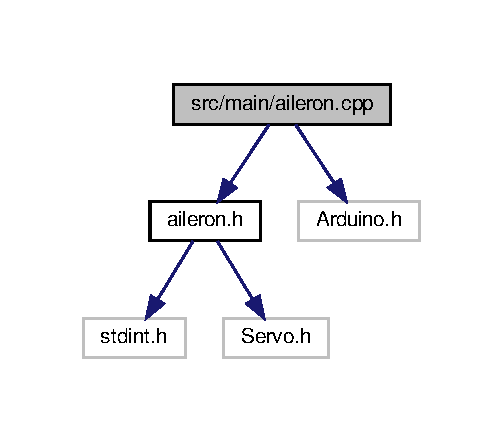
\includegraphics[width=242pt]{aileron_8cpp__incl}
\end{center}
\end{figure}


\subsection{Detailed Description}
Definition of aileron class. 

\begin{DoxyAuthor}{Author}
Valentin Mercy (\href{https://github.com/vmercy}{\tt https\+://github.\+com/vmercy}) 
\end{DoxyAuthor}
\begin{DoxyVersion}{Version}
0.\+1 
\end{DoxyVersion}
\begin{DoxyDate}{Date}
2020-\/11-\/23
\end{DoxyDate}
\begin{DoxyCopyright}{Copyright}
Copyright (c) 2020 
\end{DoxyCopyright}

\hypertarget{aileron_8h}{}\section{src/main/aileron.h File Reference}
\label{aileron_8h}\index{src/main/aileron.\+h@{src/main/aileron.\+h}}


Declaration of aileron class.  


{\ttfamily \#include $<$Arduino.\+h$>$}\newline
{\ttfamily \#include \char`\"{}Servo.\+h\char`\"{}}\newline
Include dependency graph for aileron.\+h\+:
\nopagebreak
\begin{figure}[H]
\begin{center}
\leavevmode
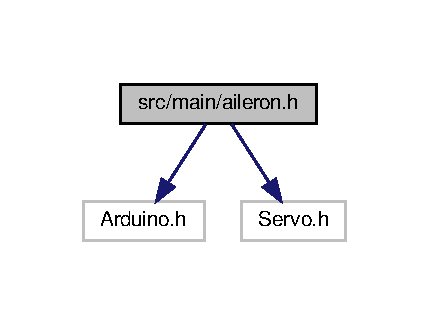
\includegraphics[width=206pt]{aileron_8h__incl}
\end{center}
\end{figure}
This graph shows which files directly or indirectly include this file\+:
\nopagebreak
\begin{figure}[H]
\begin{center}
\leavevmode
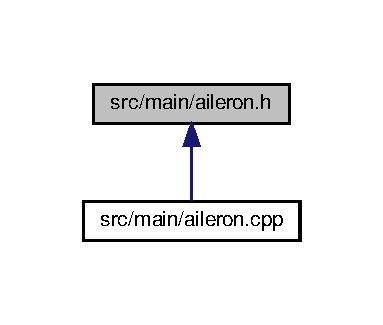
\includegraphics[width=286pt]{aileron_8h__dep__incl}
\end{center}
\end{figure}
\subsection*{Classes}
\begin{DoxyCompactItemize}
\item 
class \hyperlink{class_aileron}{Aileron}
\begin{DoxyCompactList}\small\item\em Representation of the ailerons. \end{DoxyCompactList}\end{DoxyCompactItemize}
\subsection*{Macros}
\begin{DoxyCompactItemize}
\item 
\#define \hyperlink{aileron_8h_ab6629cfdc7f2e70868390615fb77aca1}{S\+L\+O\+W\+E\+S\+T\+\_\+\+M\+O\+V\+E\+M\+E\+N\+T\+\_\+\+D\+E\+L\+AY}~100
\begin{DoxyCompactList}\small\item\em the delay between two steps (1°) for a the slowest movement available \end{DoxyCompactList}\item 
\mbox{\Hypertarget{aileron_8h_aebf857e287971afa34efe8ee8fbe5545}\label{aileron_8h_aebf857e287971afa34efe8ee8fbe5545}} 
\#define {\bfseries S\+E\+R\+V\+O\+\_\+H}
\end{DoxyCompactItemize}


\subsection{Detailed Description}
Declaration of aileron class. 

\begin{DoxyAuthor}{Author}
Valentin Mercy (\href{https://github.com/vmercy}{\tt https\+://github.\+com/vmercy}) 
\end{DoxyAuthor}
\begin{DoxyVersion}{Version}
0.\+1 
\end{DoxyVersion}
\begin{DoxyDate}{Date}
2020-\/11-\/22 
\end{DoxyDate}
\begin{DoxyCopyright}{Copyright}
Copyright (c) 2020 
\end{DoxyCopyright}


\subsection{Macro Definition Documentation}
\mbox{\Hypertarget{aileron_8h_ab6629cfdc7f2e70868390615fb77aca1}\label{aileron_8h_ab6629cfdc7f2e70868390615fb77aca1}} 
\index{aileron.\+h@{aileron.\+h}!S\+L\+O\+W\+E\+S\+T\+\_\+\+M\+O\+V\+E\+M\+E\+N\+T\+\_\+\+D\+E\+L\+AY@{S\+L\+O\+W\+E\+S\+T\+\_\+\+M\+O\+V\+E\+M\+E\+N\+T\+\_\+\+D\+E\+L\+AY}}
\index{S\+L\+O\+W\+E\+S\+T\+\_\+\+M\+O\+V\+E\+M\+E\+N\+T\+\_\+\+D\+E\+L\+AY@{S\+L\+O\+W\+E\+S\+T\+\_\+\+M\+O\+V\+E\+M\+E\+N\+T\+\_\+\+D\+E\+L\+AY}!aileron.\+h@{aileron.\+h}}
\subsubsection{\texorpdfstring{S\+L\+O\+W\+E\+S\+T\+\_\+\+M\+O\+V\+E\+M\+E\+N\+T\+\_\+\+D\+E\+L\+AY}{SLOWEST\_MOVEMENT\_DELAY}}
{\footnotesize\ttfamily \#define S\+L\+O\+W\+E\+S\+T\+\_\+\+M\+O\+V\+E\+M\+E\+N\+T\+\_\+\+D\+E\+L\+AY~100}



the delay between two steps (1°) for a the slowest movement available 

\begin{DoxyNote}{Note}
inversely proportionnal to the speed of the slowest movement 
\end{DoxyNote}

\hypertarget{battery_8cpp}{}\section{src/main/battery.cpp File Reference}
\label{battery_8cpp}\index{src/main/battery.\+cpp@{src/main/battery.\+cpp}}


definition of battery class  


{\ttfamily \#include \char`\"{}battery.\+h\char`\"{}}\newline
{\ttfamily \#include $<$Arduino.\+h$>$}\newline
Include dependency graph for battery.\+cpp\+:\nopagebreak
\begin{figure}[H]
\begin{center}
\leavevmode
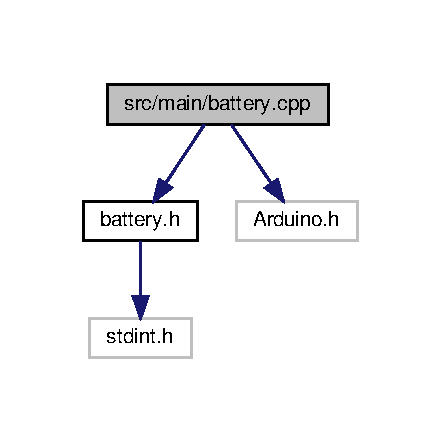
\includegraphics[width=225pt]{battery_8cpp__incl}
\end{center}
\end{figure}
\subsection*{Functions}
\begin{DoxyCompactItemize}
\item 
\mbox{\Hypertarget{battery_8cpp_a2f439a0487cb7a0c584cc43a4e72c7ac}\label{battery_8cpp_a2f439a0487cb7a0c584cc43a4e72c7ac}} 
float {\bfseries map\+Float} (float base, float min\+Base, float max\+Base, float new\+Min, float new\+Max)
\end{DoxyCompactItemize}


\subsection{Detailed Description}
definition of battery class 

\begin{DoxyAuthor}{Author}
Valentin Mercy (\href{https://github.com/vmercy}{\tt https\+://github.\+com/vmercy}) 
\end{DoxyAuthor}
\begin{DoxyVersion}{Version}
0.\+1 
\end{DoxyVersion}
\begin{DoxyDate}{Date}
2020-\/11-\/23
\end{DoxyDate}
\begin{DoxyCopyright}{Copyright}
Copyright (c) 2020 
\end{DoxyCopyright}

\hypertarget{battery_8h}{}\section{src/main/battery.h File Reference}
\label{battery_8h}\index{src/main/battery.\+h@{src/main/battery.\+h}}


declaration of battery class  


{\ttfamily \#include $<$Arduino.\+h$>$}\newline
{\ttfamily \#include \char`\"{}math\+\_\+functions.\+h\char`\"{}}\newline
Include dependency graph for battery.\+h\+:\nopagebreak
\begin{figure}[H]
\begin{center}
\leavevmode
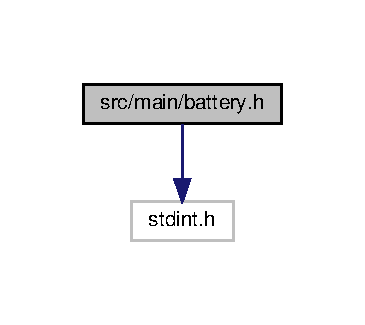
\includegraphics[width=211pt]{battery_8h__incl}
\end{center}
\end{figure}
This graph shows which files directly or indirectly include this file\+:\nopagebreak
\begin{figure}[H]
\begin{center}
\leavevmode
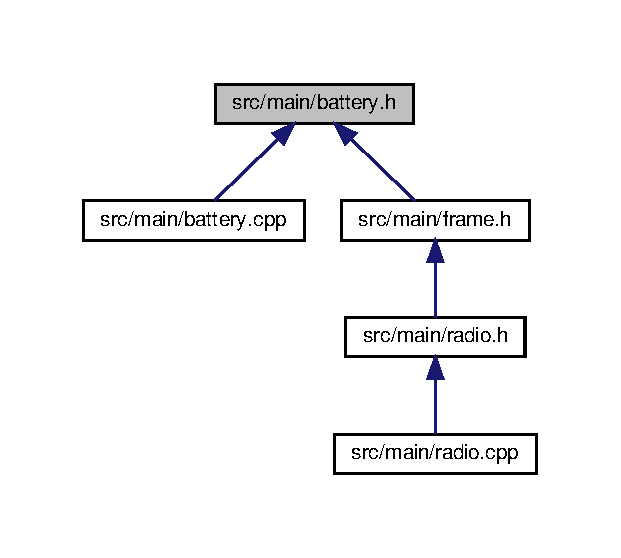
\includegraphics[width=298pt]{battery_8h__dep__incl}
\end{center}
\end{figure}
\subsection*{Classes}
\begin{DoxyCompactItemize}
\item 
class \hyperlink{class_battery}{Battery}
\end{DoxyCompactItemize}
\subsection*{Macros}
\begin{DoxyCompactItemize}
\item 
\mbox{\Hypertarget{battery_8h_af81c563d212b04612a2fdf09f5b2957c}\label{battery_8h_af81c563d212b04612a2fdf09f5b2957c}} 
\#define {\bfseries L\+I\+P\+O\+\_\+1S}~1
\item 
\mbox{\Hypertarget{battery_8h_a0ff9eb1042b121287d6abfe776ec1a8c}\label{battery_8h_a0ff9eb1042b121287d6abfe776ec1a8c}} 
\#define {\bfseries L\+I\+P\+O\+\_\+2S}~2
\item 
\mbox{\Hypertarget{battery_8h_a194fd11d79140854ebb63b4aae64f105}\label{battery_8h_a194fd11d79140854ebb63b4aae64f105}} 
\#define {\bfseries L\+I\+P\+O\+\_\+3S}~3
\item 
\mbox{\Hypertarget{battery_8h_adb9cf7290df946a808d907fd52b36adf}\label{battery_8h_adb9cf7290df946a808d907fd52b36adf}} 
\#define {\bfseries L\+I\+P\+O\+\_\+4S}~4
\item 
\mbox{\Hypertarget{battery_8h_a96a8f65f4f6e996672b62adfe98d7c46}\label{battery_8h_a96a8f65f4f6e996672b62adfe98d7c46}} 
\#define {\bfseries L\+I\+P\+O\+\_\+5S}~5
\item 
\mbox{\Hypertarget{battery_8h_a62ca371673d32217c9314773078b55ee}\label{battery_8h_a62ca371673d32217c9314773078b55ee}} 
\#define {\bfseries L\+I\+P\+O\+\_\+6S}~6
\item 
\mbox{\Hypertarget{battery_8h_ad5ec179af884bf5d81f7d7d277ad72d0}\label{battery_8h_ad5ec179af884bf5d81f7d7d277ad72d0}} 
\#define {\bfseries L\+I\+P\+O\+\_\+\+L\+O\+W\+E\+S\+T\+\_\+\+V\+O\+L\+T\+A\+GE}~3.\+3
\item 
\mbox{\Hypertarget{battery_8h_a01732358c09897aadb81cf1e07a73eca}\label{battery_8h_a01732358c09897aadb81cf1e07a73eca}} 
\#define {\bfseries L\+I\+P\+O\+\_\+\+H\+I\+G\+H\+E\+S\+T\+\_\+\+V\+O\+L\+T\+A\+GE}~4.\+2
\item 
\mbox{\Hypertarget{battery_8h_a65d999b485fd49b24b03c98367813603}\label{battery_8h_a65d999b485fd49b24b03c98367813603}} 
\#define {\bfseries B\+A\+T\+T\+E\+R\+Y\+\_\+\+C\+E\+L\+L\+\_\+\+A\+L\+E\+R\+T\+\_\+\+V\+O\+L\+T\+A\+GE}~3.\+5
\item 
\mbox{\Hypertarget{battery_8h_a3d0dbddf2f4fe415ee4c5bf20d12dc37}\label{battery_8h_a3d0dbddf2f4fe415ee4c5bf20d12dc37}} 
\#define {\bfseries B\+A\+T\+T\+E\+R\+Y\+\_\+\+C\+E\+L\+L\+\_\+\+C\+R\+I\+T\+I\+C\+A\+L\+\_\+\+V\+O\+L\+T\+A\+GE}~3.\+4
\item 
\mbox{\Hypertarget{battery_8h_af5eb7e3dc57a2c282b06f32e51970839}\label{battery_8h_af5eb7e3dc57a2c282b06f32e51970839}} 
\#define {\bfseries A\+N\+A\+L\+O\+G\+\_\+\+R\+EF}~5.\+0
\item 
\mbox{\Hypertarget{battery_8h_a38b266fc2a691a397cb0739a9e19c0a1}\label{battery_8h_a38b266fc2a691a397cb0739a9e19c0a1}} 
\#define {\bfseries A\+N\+A\+L\+O\+G\+\_\+\+P\+R\+E\+C\+I\+S\+I\+ON}~1023
\item 
\mbox{\Hypertarget{battery_8h_a2674a2c5313fff69210125ef15558bf7}\label{battery_8h_a2674a2c5313fff69210125ef15558bf7}} 
\#define {\bfseries N\+B\+\_\+\+S\+A\+M\+P\+L\+E\+S\+\_\+\+B\+A\+T\+T\+E\+RY}~10
\item 
\mbox{\Hypertarget{battery_8h_a33fa689903e4d19edd814aa108d49a91}\label{battery_8h_a33fa689903e4d19edd814aa108d49a91}} 
\#define {\bfseries D\+E\+L\+A\+Y\+\_\+\+S\+A\+M\+P\+L\+E\+S\+\_\+\+B\+A\+T\+T\+E\+RY}~500
\end{DoxyCompactItemize}


\subsection{Detailed Description}
declaration of battery class 

\begin{DoxyAuthor}{Author}
Valentin Mercy (\href{https://github.com/vmercy}{\tt https\+://github.\+com/vmercy}) 
\end{DoxyAuthor}
\begin{DoxyVersion}{Version}
0.\+1 
\end{DoxyVersion}
\begin{DoxyDate}{Date}
2020-\/11-\/21
\end{DoxyDate}
\begin{DoxyCopyright}{Copyright}
Copyright (c) 2020 
\end{DoxyCopyright}

\hypertarget{motor_8cpp}{}\section{src/main/motor.cpp File Reference}
\label{motor_8cpp}\index{src/main/motor.\+cpp@{src/main/motor.\+cpp}}


Definition of motor class.  


{\ttfamily \#include \char`\"{}motor.\+h\char`\"{}}\newline
{\ttfamily \#include $<$Arduino.\+h$>$}\newline
Include dependency graph for motor.\+cpp\+:
\nopagebreak
\begin{figure}[H]
\begin{center}
\leavevmode
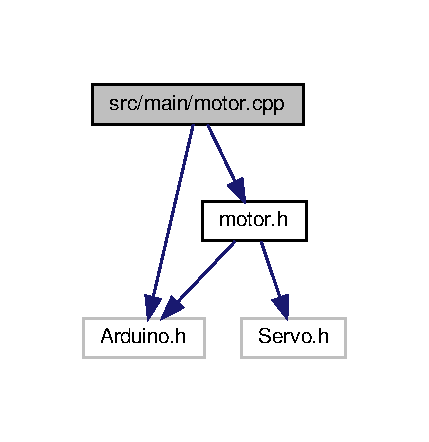
\includegraphics[width=240pt]{motor_8cpp__incl}
\end{center}
\end{figure}


\subsection{Detailed Description}
Definition of motor class. 

\begin{DoxyAuthor}{Author}
Valentin Mercy (\href{https://github.com/vmercy}{\tt https\+://github.\+com/vmercy}) 
\end{DoxyAuthor}
\begin{DoxyVersion}{Version}
0.\+1 
\end{DoxyVersion}
\begin{DoxyDate}{Date}
2020-\/11-\/23
\end{DoxyDate}
\begin{DoxyCopyright}{Copyright}
Copyright (c) 2020 
\end{DoxyCopyright}

\hypertarget{motor_8h}{}\section{src/main/motor.h File Reference}
\label{motor_8h}\index{src/main/motor.\+h@{src/main/motor.\+h}}


Declaration of motor class.  


{\ttfamily \#include $<$Arduino.\+h$>$}\newline
{\ttfamily \#include $<$Servo.\+h$>$}\newline
Include dependency graph for motor.\+h\+:
\nopagebreak
\begin{figure}[H]
\begin{center}
\leavevmode
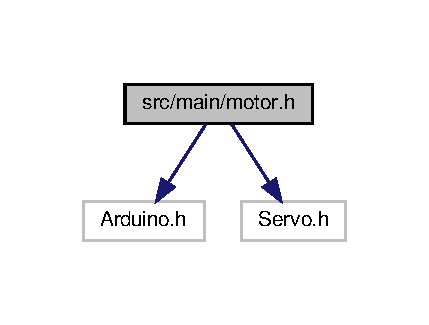
\includegraphics[width=206pt]{motor_8h__incl}
\end{center}
\end{figure}
This graph shows which files directly or indirectly include this file\+:\nopagebreak
\begin{figure}[H]
\begin{center}
\leavevmode
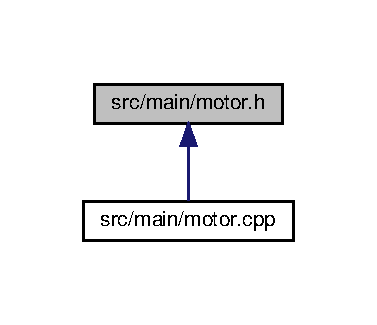
\includegraphics[width=181pt]{motor_8h__dep__incl}
\end{center}
\end{figure}
\subsection*{Classes}
\begin{DoxyCompactItemize}
\item 
class \hyperlink{class_motor}{Motor}
\begin{DoxyCompactList}\small\item\em Representation of the brushless motor. \end{DoxyCompactList}\end{DoxyCompactItemize}
\subsection*{Macros}
\begin{DoxyCompactItemize}
\item 
\mbox{\Hypertarget{motor_8h_ac2cd96d53dd3ba6407db6766c3d92b26}\label{motor_8h_ac2cd96d53dd3ba6407db6766c3d92b26}} 
\#define {\bfseries M\+A\+X\+\_\+\+S\+P\+E\+ED}~80
\item 
\mbox{\Hypertarget{motor_8h_a468208c9ffd3c1a33492c453463e82cd}\label{motor_8h_a468208c9ffd3c1a33492c453463e82cd}} 
\#define {\bfseries A\+N\+T\+I\+\_\+\+A\+R\+M\+\_\+\+S\+P\+E\+ED}~50
\item 
\mbox{\Hypertarget{motor_8h_aebf857e287971afa34efe8ee8fbe5545}\label{motor_8h_aebf857e287971afa34efe8ee8fbe5545}} 
\#define {\bfseries S\+E\+R\+V\+O\+\_\+H}
\end{DoxyCompactItemize}


\subsection{Detailed Description}
Declaration of motor class. 

\begin{DoxyAuthor}{Author}
Valentin Mercy (\href{https://github.com/vmercy}{\tt https\+://github.\+com/vmercy}) 
\end{DoxyAuthor}
\begin{DoxyVersion}{Version}
0.\+1 
\end{DoxyVersion}
\begin{DoxyDate}{Date}
2020-\/11-\/21
\end{DoxyDate}
\begin{DoxyCopyright}{Copyright}
Copyright (c) 2020 
\end{DoxyCopyright}

%--- End generated contents ---

% Index
\backmatter
\newpage
\phantomsection
\clearemptydoublepage
\addcontentsline{toc}{chapter}{Index}
\printindex

\end{document}
